\documentclass[../main.tex]{subfiles}

\begin{document}

\chapter{Đọc thơ Apollinaire - Ở biên giới của vô biên và tương lai}

\begin{subtitle}

(90 năm ngày Guillaume Apollinaire từ trần 9/11/1918 - 2008)

\end{subtitle}

\begin{metadata}

\begin{flushright}7.8.2008\end{flushright}

Hoàng Hưng

Nguồn: Kiến thức Ngày nay ngày 30.7.2008

\end{metadata}

\begin{multicols}{2}

\begin{figure}
	\centering
	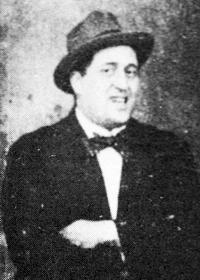
\includegraphics[width=\textwidth]{../img/tho070808_1.jpg}
	\caption{Guillaume Apollinaire 1914}
\end{figure}
 Hầu như chắc chắn rằng, bất kỳ người Pháp nào hôm nay nghe nhắc tới Apollinaire là có thể đọc liền: “Sous le pont Mirabeau coule la Seine/ et nos amours…” (Dưới cầu Mirabeau trôi dòng sông Seine/ và những cuộc tình của chúng mình...). Vào năm 1965, gần 40 năm sau ngày thi sĩ ra đi, đủ thời gian để người bạn André Billy của ông khẳng định: “Guillaume Apollinaire là nhà thơ cuối cùng được các cậu trai cô gái thuộc thơ”. Vậy mà, lúc \textit{Rượu} (Alcools), tập thơ đầu tay của Apo ra đời, nó đã hứng nhiều lời chê bai rẻ rúng, chẳng hạn nhà văn có uy thuở ấy Georges Duhamel đã phán: (tập thơ) “có đặc tính của hàng đồng nát”. 
 
Sự đa dạng của Apollinaire khiến Jacques Gaucheron ví ông như một “ngôi sao” (étoile: chỗ đất thưa cây trong rừng, từ đó tỏa ra nhiều lối mòn) của thơ Pháp thế kỷ 20. 
 
 Đại chúng thì đắm đuối với những vần điệu dặt dìu của “Cầu Mirabeau”, “Thu ốm”, “Giã từ”... Quyền lực quyến rũ của nhạc tính kiểu Nerval, Verlaine... được Apollinaire làm mới bằng những xung động bộc phát, hồn nhiên, bất ngờ, trong câu thơ đã bắt đầu có giọng văn xuôi dù số âm tiết vẫn đều đặn, hoặc là câu thơ tự do có vần. 

 \begin{figure}
	\centering
	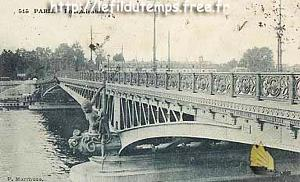
\includegraphics[width=\textwidth]{../img/tho070808_2.jpg}
	\caption{Cầu Mirabeau}
\end{figure}
 \begin{blockquote}
        
Yêu thế mùa ơi yêu tiếng mùa xôn xao        
Những trái rụng không chờ tay hái	        
Gió và rừng khóc mãi        
Cạn dòng thu từng lá lá theo nhau... 
	(“Thu ốm”) 
 \end{blockquote}
 
Nếu chỉ như vậy, Apollinaire cũng là một tiếng “nai gộ” kéo dài thêm hoàng hôn mùa “những bàn tay lá rụng” mà thôi. 
 
Nhưng “mặt trời hừng hực” của ngày mới đã mọc trong thơ anh. 
 
Một cuộc “cách mạng mỹ học” đã xảy ra từ cuộc gặp gỡ lịch sử của Apollinaire với Picasso và những thi sĩ họa sĩ trẻ tứ xứ tập họp quanh xưởng vẽ Bateau - Lavoir. 
 
 \begin{figure}
	\centering
	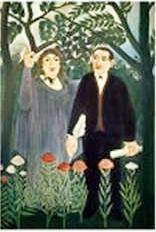
\includegraphics[width=\textwidth]{../img/tho070808_3.jpg}
	\caption{Apo và Nàng Thơ (tranh của Henri Rousseau)}
\end{figure}
 Cuồng nhiệt với hàng loạt các bài báo tung hô tinh thần hội họa mới (thường được gọi là “chủ nghĩa hiện đại” - modernisme): Lập thể (cubisme, với Picasso, Braque, Léger...) Ngây thơ (peinture naive, mà Le douanier Rousseau là bậc thầy), Duy sắc (orphisme, danh từ do chính Apollinaire đặt ra, với Delaunay...), Apollinaire cũng chân thành đoạn tuyệt “phép thơ xưa”: 
\begin{blockquote}
        
Hãy tha thứ cho tôi ngu dại        
Hãy tha thứ cho tôi không còn biết phép thơ xưa 
	(“Thời sắp cưới”) 

\end{blockquote}
 
Thực ra, Apollinaire không đơn giản như những gì ông tuyên bố. Tập \textit{Rượu }thể hiện rõ sự dao động giữa những mỹ cảm “cũ” và “mới”, sự lưỡng lự giữa thơ và văn xuôi. Nắm rất vững “phép thơ xưa” nhưng nhiều lúc nhà thơ đổi mới bằng cách làm cho nó nháo nhào. 
 
Quan trọng nhất là nhận thức về một thẩm mỹ mới được chỉ đạo bởi cái mà nhà thơ gọi là “lý trí uyển chuyển”, “lý trí kép” hay “lý trí hừng hực” của thời đại công nghiệp: 
\begin{blockquote}
        
Lý trí kép ở ngoài tầm cái đẹp 
 	Mà Hy Lạp chưa biết phương Đông cũng chưa        
... Biển cả lần lần gặm lục địa xưa 
	(“Tháng hái nho”) 

\end{blockquote}
 
Có thể nói bài thơ dài “Vùng” (Zone) được chọn để mở đầu tập \textit{Rượu} bộc lộ khá đầy đủ “tinh thần mới” của Apollinaire, tuy ông không đi theo một trường phái nào trong các trường phái cách tân như vị lai (futurisme), đồng hiện (simultanéisme)... nở rộ thi đàn Pháp đầu thế kỷ. Câu thơ - văn - xuôi dài dằng dặc lổn nhổn cái thường ngày (không loại trừ cái dung tục, nhơ bẩn \footnote{
Trong bản thảo đầu tiên của “Vùng” có câu: “Hôm nay tôi bước giữa Paris những người đàn bà vấy máu kinh nguyệt chảy đỏ các rãnh nước...”} ) vẫn còn được bảo hiểm bằng các cặp vần chân; tháp Eiffel (mà đa số các nhà hàn lâm cuối thế kỷ 19 đã nhân danh văn hóa Pháp để phủ quyết như một quái vật bằng sắt) còn được làm mềm, làm cũ đi trong lốt ẩn dụ một cô gái chăn cừu; những cảm hứng Kitô giáo và thần thoại Hy La vẫn cho máy móc của thời công nghiệp mượn hồn... Song cái cốt lõi hiện đại của bài thơ có lẽ không nằm ở việc đưa vào thơ trữ tình các vật thể thời thượng như xe hơi, máy bay... (cũng như “những bông hồng của điện lực vẫn còn mở trong khu vườn ký ức tôi”, “ngũ quan anh chụp hình màu em...” đầy rẫy trong các bài thơ khác). Sự phá vỡ cấu trúc liền mạch đơn tuyến không gian, thời gian, phá vỡ tính thống nhất đơn chủ đề, đơn tâm trạng và đơn giọng điệu của một bài thơ trữ tình truyền thống có thể đáng coi là yếu tố hiện đại quan trọng nhất của \textit{Vùng}. Không còn bài thơ như một tựu thành cô đặc của cảm xúc, đây là một dòng triền miên tùy hứng liên tưởng nhảy cóc hiện tại - quá khứ - hiện tại. Bức tranh đời sống bên ngoài xen hồi ức và tâm trạng cá nhân, tiếng kêu thất tình xen bình luận tôn giáo và mỹ học... “Cái Tôi” vừa là chủ thể vừa biến thành khách thể được quan sát: 
\begin{blockquote}
        
Tôi đã sống như thằng điên và đã đánh mất thời gian        
Mi không còn dám nhìn hai bàn tay và lúc nào tôi cũng muốn nức nở        
Khóc cho mi cho người tôi yêu và tất cả những gì làm mi khiếp sợ 

\end{blockquote}
 
Cái đặc tính “hàng đồng nát” mà những người gắn bó với truyền thống lên án đã chứa ở bề sâu của nó những gì sẽ trở thành hướng đạo cả nền thơ hiện đại sau này: Tính đồng hiện, cái ngẫu nhiên gây bất ngờ kinh ngạc, tham vọng mở rộng biên giới thơ để nó có thể thu nạp không những văn xuôi mà cả các kỹ thuật âm nhạc (phối nhiều bè), hội họa (xé dán - collage) và điện ảnh (cắt ráp - montage)... 
 
Chỉ có một sức mạnh có thể liên kết tất cả những cái xem ra rất rời rạc như thế: đó là xúc động thơ hướng nội. Như một từ trường mạnh, xúc động thơ hướng nội nhiễm từ tất cả những vụn vặt vô nghĩa tản mác của thực tại , kết chúng lại trong đường sức tâm trạng. Trước khi viết \textit{Vùng} ít lâu, bài “Du khách” (Le Voyageur), một trong số bài thơ có sức ám ảnh sâu nhất của Apollinaire, đã được ông ứng tác với sự tham gia của bạn mình là Fernand Fleuret khi hai người đi bộ từ cổng Thư viện Quốc gia, qua hai phố Richelieu và Notre Dame de Lorette. Thực ra “những bài ca nhồi nhét”, “những bài than van dân dã không đầu không cuối” (như nhận xét của Fleuret) ấy đã vụt ra từ những ám ảnh tích tụ trong cuộc đời lang bạt của một chàng “ngoại kiều” đã nhiều đau khổ vì tình. 
\begin{blockquote}
        
Hai thủy thủ không bao giờ rời nhau        
Hai thủy thủ không bao giờ nói với nhau        
Người trẻ hơn ngã nghiêng mà chết 
	(“Du khách”) 

\end{blockquote}
 
Tập \textit{Rượu} đầy những ẩn ngữ kiểu ấy. Chúng khêu gợi sự ham muốn giải mã, đồng thời lại dẫn dụ người ta để tâm trí bập bềnh trong tình trạng nửa mờ nửa tỏ. Sức mạnh của xúc động thơ hướng nội đã biến những gì có lẽ là kỷ niệm rất riêng tư của Apollinaire thành những biểu tượng lơ lửng ám ảnh tâm linh mọi người. Sức cám dỗ lâu dài của nhiều bài thơ trong tập \textit{Rượu} có lẽ ở vẻ bí ẩn \footnote{
André Billy cho rằng cái thần bí trong thơ Apollinaire bắt nguồn từ nguồn gốc Slave và tuổi thơ học nội trú trong trường Công giáo của nhà thơ.}  của những hình ảnh nhiều chất siêu thực trong đó. 
 
 \begin{figure}
	\centering
	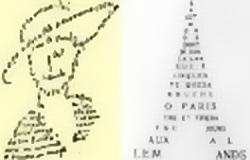
\includegraphics[width=\textwidth]{../img/tho070808_4.jpg}
	\caption{Thư đồ}
\end{figure}
 Gần một thế kỷ đã qua, các thí nghiệm về kỹ thuật thơ của Apollinaire (như sắp xếp bài thơ thành hình vẽ...) không chứng tỏ được sức sống của nó, tuy nhiên tập thơ mang tên \textit{Calligrammes}, tập họp các bài thơ viết trước và trong Thế chiến thứ Nhất, lại tồn tại nhờ những cảm nhận mãnh liệt và suy tư sâu rộng của nhà thơ về một thế giới mới trong cơn chuyển dạ sẽ làm biến đổi tận cùng đời sống nhân loại. Trong đêm trước ngày nước Pháp tổng động viên đánh Đức, trên chiếc xe hơi nhỏ chở nhà thơ từ biên giới trở về Paris, ông đã khải thị những viễn cảnh bi tráng của thời đại mới: 
\begin{blockquote}
        
Chúng tôi chào từ biệt cả một thời đại        
Những tên khổng lồ giận dữ vươn mình trên châu Âu        
Những con đại bàng rời tổ đợi mặt trờI        
Những con cá háu ăn ngoi lên từ các vực sâu        
Những dân tộc chạy đến nhau để hiểu nhau tận đáy        
Những người chết run sợ trong nơi trú ngụ tối tăm         
(“Chiếc xe hơi nhỏ”) 

\end{blockquote}
 
Vẫn là mạch cảm hứng vũ trụ lồng lộng không gian Kinh Thánh của một số trường thi trong tập \textit{Rượu}, tiêu biểu nhất là “Tháng hái nho” (Vendémiaire):  
\begin{blockquote}
        
Tôi say vì đã uống tất cả vũ trụ         
Trên bến tàu đứng đấy tôi nhìn làn nước chảy và những chiếc xuồng ngủ         
Hãy nghe tôi, tôi là cổ họng của Paris         
Và tôi sẽ còn uống vũ trụ nữa nếu như tôi thích...  

\end{blockquote}
 
Cảm hứng ấy khi thì mang vẻ huy hoàng của \textit{Sáng thế ký} khi thì đầy không khí kỳ bí của sách \textit{Khải huyền}. 
  
Bốn tháng sau khi nước Pháp tuyên chiến, Guillaume tình nguyện đăng lính để chiến đấu như một công dân Pháp. Người ta sẽ nói về thái độ hời hợt đối với chiến tranh của anh nhà thơ - hạ sĩ từng ca tụng “Đẹp sao hỏa châu rực rỡ trời đêm”. Nhưng hóa ra điều choán gần hết tâm trí của Apollinaire trong thời gian này lại là viễn ảnh của một tương lai chưa từng có, tạo bởi sức mạnh phi thường của trí tuệ loài người mà cuộc đại chiến đã bộc lộ các khả năng. 
\begin{blockquote}
        
Chiến tranh trước nhất sẽ là         
Thấy xa thật rõ         
Là thấy hết         
Từ gần         
Và tất cả mang một tên mới        
(“Chiến thắng”) 

\end{blockquote}
 
Trước viễn cảnh ấy, Apollinaire nhiều lần hùng hồn tuyên ngôn bằng thơ về sứ mệnh “tiên tri” của nhà thơ, việc “tìm kiếm một ngôn ngữ mới” thay thế cho “Những thứ tiếng già nua sắp chết / Thực tình chỉ do thói quen và thiếu can đảm / Mà người ta còn dùng để phục vụ thơ”. Nhưng cũng không ít lần ông phải kêu lên những lời thống thiết về thân phận của những kẻ “luôn chiến đấu ở biên giới / của vô biên và tương lai”: 
\begin{blockquote}
        
Nhưng hãy cười tôi hãy cười tôi        
Hỡi người muôn nơi nhất là người ở đây         
Vì có bao điều tôi không dám nói         
Bao điều các anh không để cho tôi nói         
Xin hãy thương tôi        
(“Nàng tóc hung xinh đẹp”) 

\end{blockquote}
 
Xưa nay trên thế giới, Đông lẫn Tây, không ít nhà thơ dùng thơ để tuyên ngôn về thơ, song “Nàng tóc hung xinh đẹp” (La Jolie Rousse) của Apollinaire là một bài thơ thực sự, nó phơi bầy niềm say mê và nỗi đau đáu của kẻ trên đường hành hương tìm chân lý nghệ thuật, y như gã si tình đuổi theo bóng dáng kiều nữ, không phải những lời biện lý sắc sảo hay những kết luận sáng suốt “có sẵn đây rồi” được thông đạt bằng ngôn ngữ giàu hình ảnh và âm điệu mang hình thức thơ. (Tương tự khác biệt giữa bài thơ mang tư tưởng triết học với cái thường được gọi là “thơ triết lý”.) 
 
Ý tưởng về cái mới trong thơ, về sau được Apollinaire đúc lại trong bài nói chuyện “Tinh thần mới và các nhà thơ” năm 1917. Theo ông, nhiệm vụ của thơ là “thăm dò sự thật, tìm hiểu sự thật” để “hiểu biết rõ ràng về thời đại của mình và để mở ra những cái nhìn mới trước vũ trụ bên ngoài và bên trong”, là “tiên tri”, là sáng tạo: “Chỉ có thể gọi là nhà thơ kẻ nào phát kiến, kẻ nào sáng tạo” - trước nhất là sáng tạo một hình thức thơ bao quát được mọi phương tiện nghệ thuật như ca múa, đặc biệt là điện ảnh, để “tạo nên quyển sách nhìn được và nghe được của tương lai”. Ông coi đặc tính quan trọng nhất của “tinh thần mới” trong nghệ thuật là “sự ngạc nhiên”. 
 
Thực tế sáng tác của Apollinaire không thể hiện hết những chủ trương sáng tạo của ông, nhưng riêng “sự ngạc nhiên” thì đúng là cái mà thơ ông luôn luôn đạt được. Thơ ông chất đầy hình ảnh lạ, đó là sản phẩm của đôi mắt vĩnh viễn trẻ thơ háo hức nhìn thế giới, cái gì cũng bị đôi mắt ấy thu phục thành thơ một cách trực tiếp hoặc thông qua liên tưởng bất ngờ kiểu như: “Một gia đình chở đi cái mền lông màu đỏ giống như em chở trái tim” (“Vùng”) hoặc “Tim họ lung lay như cánh cửa” (“Marizibil”). Thơ ông cũng đầy câu chữ lạ, những chữ do ông tạo ra, hoặc cho nghĩa khác. Có lẽ Apollinaire là nhà thơ đầu tiên hân hoan “chơi chữ”, một cách hệ thống và có ý thức trong thơ. Thái độ của ông đối với chữ tương hợp hoàn toàn với quan niệm của ông về vai trò của màu sắc trong hội họa mới: “Không còn chỉ là việc tô màu, cuối cùng cũng không còn sự biểu nghĩa có tính biểu tượng, vì bản thân nó (màu sắc - HH) là hình thức và ánh sáng của cái được diễn tả”. 
 
Những nét chủ đạo trong “tinh thần mới” của Apollinaire đã được khai triển gần một thế kỷ qua theo những con đường khác nhau. Đặc biệt những nhà sáng lập “Chủ nghĩa siêu thực” (mà cái tên cũng do Apollinaire “chế” ra: sur-réaliste nguyên là tính từ ông dùng cho một màn kịch gây xì-căng-đan của mình vào năm 1917) nhất định coi nhà thơ đàn anh này là ông thầy của họ. Thực ra với Apollinaire, “siêu thực” chỉ có nghĩa là một cách nhìn khác đối với tự nhiên, không rập theo đúng tự nhiên, đầy năng động, giàu màu sắc mạnh, nhưng chủ nghĩa siêu thực đã lấy cảm hứng khá nhiều từ những câu thơ đầy tình cờ, trực giác và thấu thị của ông để đi vào thám hiểm thế giới tiềm thức. 
 
Nếu vai trò tiên phong trong thơ hiện đại của Apollinaire được giới văn nghệ, trí thức treo cao, thì với người đọc đông đảo, trước hết và cuối cùng ông vẫn là thi sĩ của tình yêu, đặc biệt là của những mối tình “giữa đường đứt gánh”. “Bài hát kẻ bị phụ tình” (La chanson du mal-aimé), đỉnh cao đầu tiên của thơ ông, viết năm 1903 sau khi bị cô người yêu đầu tiên Annie Pleyden đoạn tuyệt, là tập hợp nhiều khúc thơ lạ lùng, nhiều khúc rất khó hiểu, nhiều đoạn đau đớn đến mê sảng: “Tình yêu chết rồi tôi run cả người”. Rồi những nhạc điệu khi da diết khi uể oải của “Cầu Mirabeau”, “Marie”... khi khắc khoải đến “nghẹt cổ” (“Vùng”) sau sự dứt tình của Marie Laurencin. Đến mấy năm cuối đời, cảm hứng yêu đương của Apollinaire trào lên hết cỡ trong hơn hai trăm bức thư - thơ gửi từ tiền tuyến về cho nàng Lou. Thiếu phụ đầy quyến rũ ấy cho anh tận hưởng lạc thú yêu đương trong 10 ngày trước khi ra trận, rồi dứt khoát chia tay, để lại anh chàng hạ sĩ như điên như dại, đêm ngày mặt trận chỉ chứa đầy hình bóng nàng, mọi thứ xung quanh đều gợi về thân thể nàng một cách tuyệt vọng. Đến mức “Miệng em là vết thương nóng rực của lòng dũng cảm” thì thật bất ngờ và cháy bỏng, đúng là thơ tình của người sống giữa cái chết. Những vần thơ táo bạo, chân thành, mê đắm nhất ra đời trong tình huống ấy:  
\begin{blockquote}
        
Lou của anh Lou yêu của anh anh có những chiếc hôn đầy môi         
Anh đặt lên mắt lên tóc em         
Màu vàng hung khắp mọi chỗ mọi chỗ những chiếc hôn điên dại.  

\end{blockquote}
 
Có người đã gọi Apollinaire là “nhà thơ lớn của thân thể và vẻ đẹp phái nữ” (Jacques Gaucheron). Tiếng cười nhạo, sự trần trụi, nhục cảm lắm khi đi tới erotique, đó là những âm sắc mạnh làm thơ tình Apollinaire những lúc say đắm hay buồn đau nhất hoặc trở lại hình thức những khổ thơ vần điệu “cổ điển”, cũng không chung giọng với các thi sĩ lãng mạn và tượng trưng của thế kỷ trước. 
  
 


\end{multicols}
\end{document}